\documentclass[12pt, a4paper]{report}

% --- ESSENTIAL PACKAGES ---
\usepackage[utf8]{inputenc}
\usepackage[english]{babel}
\usepackage{geometry}
\usepackage{graphicx}
\usepackage{amsmath}
\usepackage{fancyhdr}
\usepackage{booktabs}
\usepackage{hyperref}
\usepackage{tikz}
\usepackage{listings} % For MATLAB code
\usetikzlibrary{shapes.geometric, arrows.meta, positioning, calc, fit}

% --- PAGE AND HEADER CONFIGURATION ---
\geometry{a4paper, margin=2.5cm, headheight=15pt}
\pagestyle{fancy}
\fancyhf{}
\fancyhead[L]{Low Voltage Electrical Installation Project}
\fancyhead[R]{TechnoParque Almería}
\fancyfoot[C]{\thepage}
\renewcommand{\headrulewidth}{0.4pt}
\fancypagestyle{plain}{
  \fancyhf{} % Clear headers and footers for chapter start pages
  \renewcommand{\headrulewidth}{0pt} % No line
}

% --- HYPERLINK CONFIGURATION ---
\hypersetup{
    colorlinks=true,
    linkcolor=blue,
    urlcolor=cyan,
}

% --- MATLAB CODE LISTING STYLE ---
\definecolor{codegreen}{rgb}{0,0.6,0}
\definecolor{codegray}{rgb}{0.5,0.5,0.5}
\definecolor{codepurple}{rgb}{0.58,0,0.82}
\definecolor{backcolour}{rgb}{0.95,0.95,0.92}

\lstdefinestyle{mystyle}{
    backgroundcolor=\color{backcolour},   
    commentstyle=\color{codegreen},
    keywordstyle=\color{blue},
    numberstyle=\tiny\color{codegray},
    stringstyle=\color{codepurple},
    basicstyle=\footnotesize\ttfamily,
    breakatwhitespace=false,         
    breaklines=true,                 
    captionpos=b,                    
    keepspaces=true,                 
    numbers=left,                    
    numbersep=5pt,                  
    showspaces=false,                
    showstringspaces=false,
    showtabs=false,                  
    tabsize=2,
    literate=*{_}{{\_}}{1} % FIX: Treat underscore as a literal character
}
\lstset{style=mystyle}

% =================================================================
% --- DOCUMENT START ---
% =================================================================
\begin{document}

% --- TITLE PAGE ---
\begin{titlepage}
    \centering
    \vspace*{2cm}
    {\Huge \textbf{TECHNICAL PROJECT}}
    \vspace{1.5cm}
    {\Large \textbf{Low Voltage Electrical Installation for a Technology Park Supply}}
    \vspace{2cm}
    {\Large \textbf{TechnoParque Almería}}
    \vspace{\fill}
    {\large Promoter: [Your Name/Company]}
    \vfill
    {\large Date: October 2025}
\end{titlepage}

% --- TABLE OF CONTENTS ---
\tableofcontents
\newpage

% =================================================================
\chapter{Project Objective}
\label{chap:objeto}
The purpose of this document is to describe and justify, on a technical and regulatory level, the design of the Low Voltage (LV) electrical distribution installation for the "TechnoParque Almería" technology park.

The installation originates from several Transformation Centers (TCs) supplied by a Medium Voltage (MV) ring network, and distributes energy to the various consumers in the park, including industrial facilities, an office building, a technology museum, a residential area, and the public lighting system.

The design has been carried out following the prescriptions of the Low Voltage Electrotechnical Regulation (REBT) and its Complementary Technical Instructions (ITC-BT).

\chapter{Applicable Regulations}
\label{chap:normativa}
The design, calculation, and execution of the installation described in this project are governed by the following regulations:
\begin{itemize}
    \item Royal Decree 842/2002, of August 2, which approves the \textbf{Low Voltage Electrotechnical Regulation (REBT)}.
    \item Complementary Technical Instructions (ITC-BT), especially:
    \begin{itemize}
        \item \textbf{ITC-BT-04}: Documentation and commissioning of installations.
        \item \textbf{ITC-BT-06}: Overhead networks for low voltage distribution.
        \item \textbf{ITC-BT-07}: Underground networks for low voltage distribution.
        \item \textbf{ITC-BT-09}: Outdoor lighting installations.
        \item \textbf{ITC-BT-19}: Indoor or receiver installations. General prescriptions.
        \item \textbf{ITC-BT-10}: Load forecasting for low voltage supplies.
    \end{itemize}
    \item Specific regulations of the local distribution company (to be specified).
\end{itemize}

\chapter{General Description of the Installation}
\label{chap:descripcion}
The electrical infrastructure of TechnoParque has been designed to ensure high reliability and supply quality, consistent with the needs of a technological and business environment. The general architecture is based on the diagram in Figure \ref{fig:esquema_general} (see Chapter \ref{chap:planos}).

The installation consists of the following main elements:
\begin{enumerate}
    \item \textbf{Medium Voltage (MV) Distribution Network:} An underground ring network at 20 kV that interconnects several Transformation Centers. This topology ensures the continuity of supply to the TCs in case of a fault in a section of the ring.
    \item \textbf{Transformation Centers (TCs):} Two prefabricated centers (TC-1 and TC-2) of 400 kVA each. They are responsible for reducing the voltage from 20 kV to 400/230 V for low voltage distribution.
    \item \textbf{General Feeder Lines (LGA):} Underground low voltage circuits that start from each TC to supply the General Command and Protection Panels (CGMP) of the various consumers. The building connection cables will be Copper with XLPE insulation (type RZ1-K 0.6/1 kV), installed in buried conduits.
    \item \textbf{Consumers:}
    \begin{itemize}
        \item Industrial Facilities (x3).
        \item Office Building.
        \item Technology Museum.
        \item Residential Area.
        \item Public Lighting.
    \end{itemize}
\end{enumerate}

\chapter{Load Forecasting}
\label{chap:cargas}
The maximum expected power for each of the technology park's receivers is detailed below. A global power factor ($\cos \varphi$) of \textbf{0.9} is assumed for all calculations.

\subsection{Office Building}
An installed power of \textbf{20 kW} is estimated. This figure includes centralized air conditioning, multiple workstations with computer equipment, lighting, and general services.

\subsection{Industrial Facilities}
Three facilities are planned:
\begin{itemize}
    \item \textbf{Facility 1 (R\&D):} A power of \textbf{300 kW} is anticipated, justified by high-consumption machinery such as MRI prototypes, HPC laboratories, or large climatic chambers.
    \item \textbf{Facilities 2 \& 3 (Workshops):} A power of \textbf{75 kW} is estimated for each of these.
\end{itemize}

\subsection{Technology Museum}
For the 13,600 $\text{m}^2$ museum, an installed power of \textbf{100 kW} is estimated for lighting, air conditioning, and audiovisual equipment.

\subsection{Outdoor Lighting}
For a 1 km perimeter, 34 LED luminaires of 150 W will be installed, resulting in a total power of \textbf{5.1 kW}.

\subsection{Residential Area}
A small residential area with 10 homes is planned. ITC-BT-10 is applied with high electrification (9,200 W per home) and a simultaneity factor. The total simultaneous power is calculated to be \textbf{27.0 kW}.

\subsection{Summary Table and Total Demand}
A global simultaneity factor of \textbf{0.7} is applied to the total installed power.

\begin{table}[htbp]
    \centering
    \caption{Summary of installed power.}
    \label{tab:potencias}
    \begin{tabular}{@{}lc@{}}
        \toprule
        \textbf{Receiver} & \textbf{Power (kW)} \\ \midrule
        Office Building & 20.0 \\
        Industrial Facility 1 (R\&D) & 300.0 \\
        Industrial Facility 2 & 75.0 \\
        Industrial Facility 3 & 75.0 \\
        Technology Museum & 100.0 \\
        Outdoor Lighting & 5.1 \\
        Residential Area & 27.0 \\ \midrule
        \textbf{Total Installed} & \textbf{602.1 kW} \\ \bottomrule
    \end{tabular}
\end{table}

\begin{itemize}
    \item \textbf{Maximum simultaneous power:} $602.1 \text{ kW} \times 0.7 = \textbf{421.5 kW}$
    \item \textbf{Simultaneous apparent power:} $421.5 \text{ kW} / 0.9 = \textbf{468.3 kVA}$
\end{itemize}

\textbf{Conclusion:} The maximum expected demand of 468.3 kVA justifies the installation of two 400 kVA Transformation Centers, distributing the loads to ensure reliability and optimize the lengths of the LV lines.

\chapter{Justifying Calculations}
\label{chap:calculos}
This chapter sizes the General Feeder Lines (LGA) from the TCs to each general panel. A line voltage of 400 V and a power factor of 0.9 are assumed.

\subsection{Calculation of Nominal Currents}
The nominal current ($I_N$) for each three-phase line is calculated with the formula: $I_N = \frac{P}{\sqrt{3} \cdot U \cdot \cos \varphi}$.
\begin{itemize}
    \item \textbf{LGA R\&D Facility:} $I_N = \frac{300,000}{\sqrt{3} \cdot 400 \cdot 0.9} = 481.1 \text{ A}$
    \item \textbf{LGA Museum:} $I_N = \frac{100,000}{\sqrt{3} \cdot 400 \cdot 0.9} = 160.4 \text{ A}$
    \item \textbf{LGA Offices:} $I_N = \frac{20,000}{\sqrt{3} \cdot 400 \cdot 0.9} = 32.1 \text{ A}$
\end{itemize}

\subsection{Sizing by Voltage Drop}
Sizing is for a maximum voltage drop of 1.5\% for underground LGA (ITC-BT-07), which is 6 V. The following distances from the TC are assumed: R\&D Facility (100m), Museum (150m), Offices (80m). Copper cable is used ($\sigma = 48 \frac{m}{\Omega \cdot mm^2}$ for cables $>16mm^2$).
The minimum cross-section ($s$) is calculated with: $s = \frac{P \cdot L}{\sigma \cdot U^2 \cdot \Delta u_{\%}}$.
\begin{itemize}
    \item \textbf{LGA R\&D Facility:} $s = \frac{300,000 \cdot 100}{48 \cdot 400^2 \cdot 0.015} = 260.4 \text{ mm}^2$
    \item \textbf{LGA Museum:} $s = \frac{100,000 \cdot 150}{48 \cdot 400^2 \cdot 0.015} = 130.2 \text{ mm}^2$
    \item \textbf{LGA Offices:} $s = \frac{20,000 \cdot 80}{48 \cdot 400^2 \cdot 0.015} = 13.9 \text{ mm}^2$
\end{itemize}

\subsection{Check by Maximum Admissible Current}
It is verified if the next standard cross-section supports the nominal current. Buried installation in conduit is assumed (Method D, table 1 of ITC-BT-07) with RZ1-K(AS) cables.
\begin{itemize}
    \item \textbf{LGA R\&D Facility:} Calculated section 260.4 $\text{mm}^2$. The standard \textbf{2x(240 $\text{mm}^2$)} in parallel per conductor is chosen. $I_{adm} \approx 2 \times 364 = 728$ A. Since $481.1 \text{ A} < 728 \text{ A}$, it is valid.
    \item \textbf{LGA Museum:} Calculated section 130.2 $\text{mm}^2$. The standard \textbf{150 $\text{mm}^2$} is chosen. $I_{adm} = 286$ A. Since $160.4 \text{ A} < 286 \text{ A}$, it is valid.
    \item \textbf{LGA Offices:} Calculated section 13.9 $\text{mm}^2$. The standard \textbf{16 $\text{mm}^2$} is chosen. $I_{adm} = 85$ A. Since $32.1 \text{ A} < 85 \text{ A}$, it is valid.
\end{itemize}

\subsection{Selection of Protections}
A General Automatic Circuit Breaker (IGA) is chosen for each LGA with a nominal rating ($I_n$) that satisfies $I_N \le I_n \le I_{adm}$.
\begin{itemize}
    \item \textbf{LGA R\&D Facility:} $I_N=481.1$ A. A \textbf{500 A} IGA is chosen.
    \item \textbf{LGA Museum:} $I_N=160.4$ A. A \textbf{200 A} IGA is chosen.
    \item \textbf{LGA Offices:} $I_N=32.1$ A. A \textbf{40 A} IGA is chosen.
\end{itemize}


\chapter{Design Methodology with MATLAB}
\label{chap:matlab}
The design of the TechnoParque Almería electrical installation has been fundamentally supported by a suite of calculation and analysis tools developed in MATLAB. This approach has allowed us to go beyond manual calculations, bringing efficiency, precision, and optimization capabilities to the project.

\subsection{Automation and Efficiency}
The MATLAB suite automates the repetitive and complex calculations required by the REBT, such as the calculation of currents, electrical moments, and cumulative voltage drops in networks with multiple loads. This not only drastically reduces design time but also minimizes the probability of human error.

\subsection{Techno-Economic Optimization}
One of the most powerful capabilities of the suite is the optimization algorithm, implemented in the \texttt{H4\_OptimizeRadialNetwork.m} function. Instead of simply finding a valid conductor cross-section, this algorithm seeks the optimal solution. It iterates through standardized conductor cross-sections, verifying compliance with voltage drop and maximum admissible current criteria for each one. The first cross-section that meets all requirements is recommended, thus guaranteeing the most economical solution that fully satisfies the technical demands.

\subsection{Comparative Analysis of Topologies}
The modular structure of the software (Modules H, I, and J) has facilitated a rigorous comparative analysis between different network topologies. The \texttt{J5\_CompareNetworks.m} function, for example, allows for the evaluation of the same load configuration in both a radial and a ring network, providing quantitative data on:
\begin{itemize}
    \item \textbf{Voltage Quality:} Comparing voltage profiles and maximum drops.
    \item \textbf{Reliability:} Analyzing network behavior under fault conditions.
    \item \textbf{Life Cycle Cost:} Evaluating the initial cost versus the long-term cost of energy losses.
\end{itemize}
This capability is crucial for making informed engineering decisions and justifying the choice of a more reliable (and initially more expensive) topology like the ring network for this technology park.

\subsection{Visualization and Verification}
Finally, the visualization tools (\texttt{H2\_PlotRadialProfile.m}, \texttt{I2\_PlotDualFedProfile.m}, etc.) automatically generate graphs of voltage profiles, load diagrams, and single-line diagrams. These visual representations are indispensable for interpreting results, detecting potential problems (such as excessive voltage drops at intermediate points), and documenting the project in a clear and professional manner.

In summary, the MATLAB suite has served as a comprehensive tool that not only performs the calculations but also verifies regulatory compliance, optimizes the design from an economic perspective, and facilitates the understanding and justification of the adopted solutions.

\chapter{Drawings}
\label{chap:planos}
This chapter presents the simplified single-line diagrams of the installation, generated using LaTeX code for a conceptual representation.

\begin{figure}[htbp]
    \centering
    \resizebox{\textwidth}{!}{
    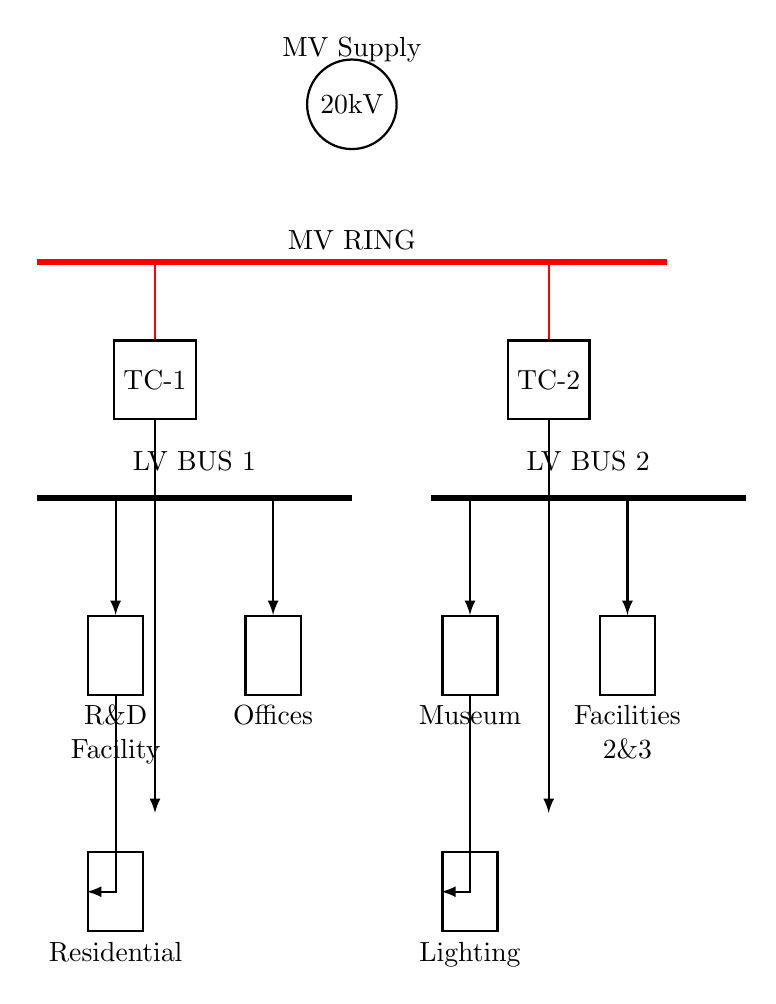
\begin{tikzpicture}[
        node distance=2.5cm and 2cm,
        source/.style={draw, circle, thick, minimum size=1cm},
        bus/.style={draw, line width=2pt},
        ct/.style={draw, thick, rectangle, minimum size=1cm},
        load/.style={draw, thick, minimum height=1cm, minimum width=0.7cm, label=below:\parbox{2cm}{\centering #1}},
        line/.style={thick},
        arrow/.style={-latex, thick}
    ]
        % Source and Main Bus
        \node[source] (mt_source) at (0,8) {20kV};
        \node at (0,8.7) {MV Supply};
        \draw[bus, red] (-4,6) -- (4,6) node[midway, above, black]{MV RING};

        % TCs
        \node[ct] (ct1) at (-2.5, 4.5) {TC-1};
        \node[ct] (ct2) at (2.5, 4.5) {TC-2};
        \draw[line, red] (ct1) -- (-2.5,6);
        \draw[line, red] (ct2) -- (2.5,6);

        % LV Buses
        \draw[bus] (-4,3) -- (0,3) node[midway, above, black, yshift=2mm]{LV BUS 1};
        \draw[bus] (1,3) -- (5,3) node[midway, above, black, yshift=2mm]{LV BUS 2};
        \draw[arrow] (ct1) -- (ct1 |- 0,-1);
        \draw[arrow] (ct2) -- (ct2 |- 1, -1);
        
        % Loads
        \node[load=R\&D Facility] (ind1) at (-3, 1) {};
        \node[load=Offices] (off) at (-1, 1) {};
        \node[load=Museum] (mus) at (1.5, 1) {};
        \node[load=Facilities 2\&3] (ind23) at (3.5, 1) {};
        \node[load=Residential] (res) at (-3, -2) {};
        \node[load=Lighting] (alum) at (1.5, -2) {};
        
        % Connections to LV Buses
        \draw[arrow] (-3,3) -- (ind1);
        \draw[arrow] (-1,3) -- (off);
        \draw[arrow] (1.5,3) -- (mus);
        \draw[arrow] (3.5,3) -- (ind23);
        
        % Connections from loads with sub-feeds
        \draw[arrow] (ind1.south) |- (res.west);
        \draw[arrow] (mus.south) |- (alum.west);

    \end{tikzpicture}
    }
    \caption{General single-line diagram of the TechnoParque installation.}
    \label{fig:esquema_general}
\end{figure}

\begin{figure}[htbp]
    \centering
    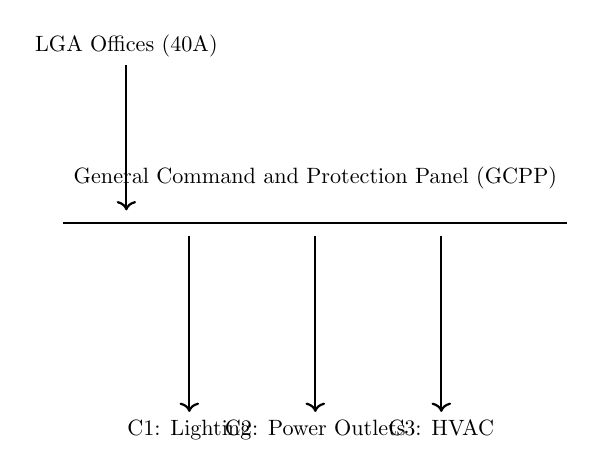
\begin{tikzpicture}[thick, scale=0.8, every node/.style={scale=0.8}]
        \draw (-1,0) -- (7,0);
        \node[above, align=center, yshift=0.4cm] at (3,0) {General Command and Protection Panel (GCPP)};
        % LGA
        \draw[->] (0,2.5) -- (0,0.2); \node[above, align=center] at (0,2.5) {LGA Offices (40A)};
        % Sub-circuits
        \draw (1,-0.2) -- (1,-2); \draw[->] (1,-2) -- (1,-3); \node[below] at (1,-3){C1: Lighting};
        \draw (3,-0.2) -- (3,-2); \draw[->] (3,-2) -- (3,-3); \node[below] at (3,-3){C2: Power Outlets};
        \draw (5,-0.2) -- (5,-2); \draw[->] (5,-2) -- (5,-3); \node[below] at (5,-3){C3: HVAC};
    \end{tikzpicture}
    \caption{Simplified single-line diagram for the Office Building.}
\end{figure}

\begin{figure}[htbp]
    \centering
    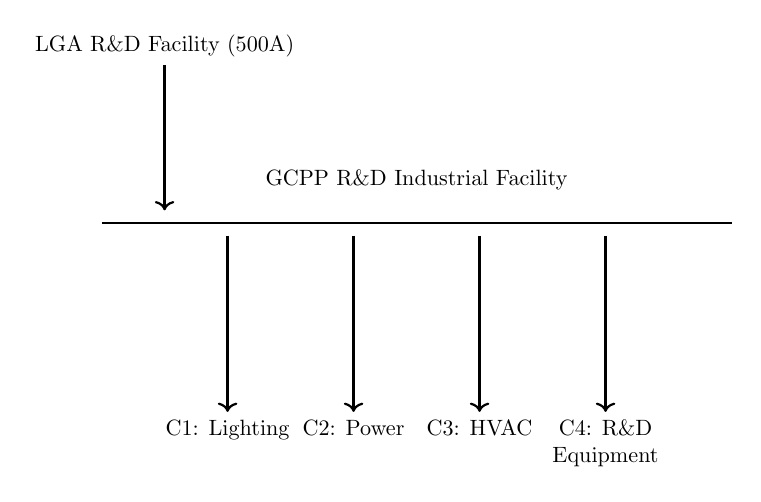
\begin{tikzpicture}[thick, scale=0.8, every node/.style={scale=0.8}]
        \draw (-1,0) -- (9,0);
        \node[above, align=center, yshift=0.4cm] at (4,0) {GCPP R\&D Industrial Facility};
        % LGA
        \draw[->] (0,2.5) -- (0,0.2); \node[above, align=center] at (0,2.5) {LGA R\&D Facility (500A)};
        % Sub-circuits
        \draw (1,-0.2) -- (1,-2); \draw[->] (1,-2) -- (1,-3); \node[below] at (1,-3){C1: Lighting};
        \draw (3,-0.2) -- (3,-2); \draw[->] (3,-2) -- (3,-3); \node[below] at (3,-3){C2: Power};
        \draw (5,-0.2) -- (5,-2); \draw[->] (5,-2) -- (5,-3); \node[below] at (5,-3){C3: HVAC};
        \draw (7,-0.2) -- (7,-2); \draw[->] (7,-2) -- (7,-3); \node[below,align=center] at (7,-3){C4: R\&D\\Equipment};
    \end{tikzpicture}
    \caption{Simplified single-line diagram for the Research Facility.}
\end{figure}

\begin{figure}[htbp]
    \centering
    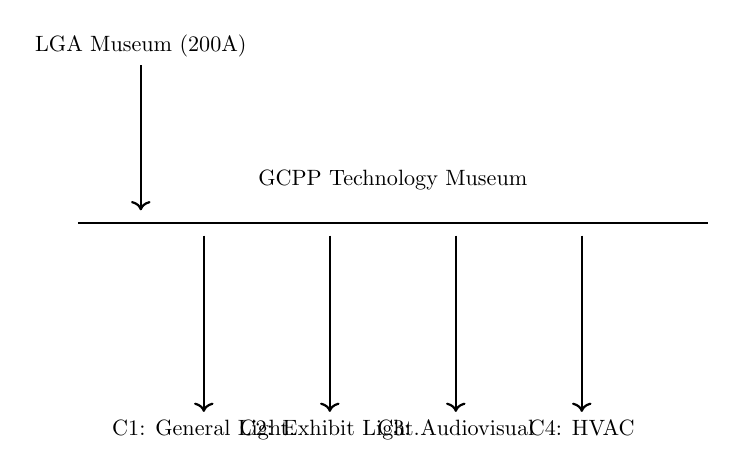
\begin{tikzpicture}[thick, scale=0.8, every node/.style={scale=0.8}]
        \draw (-1,0) -- (9,0);
        \node[above, align=center, yshift=0.4cm] at (4,0) {GCPP Technology Museum};
        % LGA
        \draw[->] (0,2.5) -- (0,0.2); \node[above, align=center] at (0,2.5) {LGA Museum (200A)};
        % Sub-circuits
        \draw (1,-0.2) -- (1,-2); \draw[->] (1,-2) -- (1,-3); \node[below] at (1,-3){C1: General Light.};
        \draw (3,-0.2) -- (3,-2); \draw[->] (3,-2) -- (3,-3); \node[below] at (3,-3){C2: Exhibit Light.};
        \draw (5,-0.2) -- (5,-2); \draw[->] (5,-2) -- (5,-3); \node[below] at (5,-3){C3: Audiovisual};
        \draw (7,-0.2) -- (7,-2); \draw[->] (7,-2) -- (7,-3); \node[below] at (7,-3){C4: HVAC};
    \end{tikzpicture}
    \caption{Simplified single-line diagram for the Technology Museum.}
\end{figure}


\end{document}

